\renewcommand{\baselinestretch}{2} \small\normalsize
\chapter{Radar Additional Stuff}

\section{Beam Width}
The beam width of an antenna is defined as the angle between the half power points in the antenna pattern. We will use a sinc antenna pattern to demonstrate this concept.

\subsection{One Way}
The one way antenna beam width, $\theta$, is simply the beam width of the forward propagating beam. The electric field amplitude in the far field of a sinc antenna pattern is given by Equation \ref{rb_eq:1} and shown in Figure \ref{rb_fig:4}.

\begin{equation}
\label{rb_eq:1}
E(\theta) = \frac{\sin\left(\frac{\pi D}{\lambda}\sin(\theta) \right)}{\frac{\pi D}{\lambda}\sin(\theta)}
\end{equation}

\begin{figure}[H]
  \begin{center}
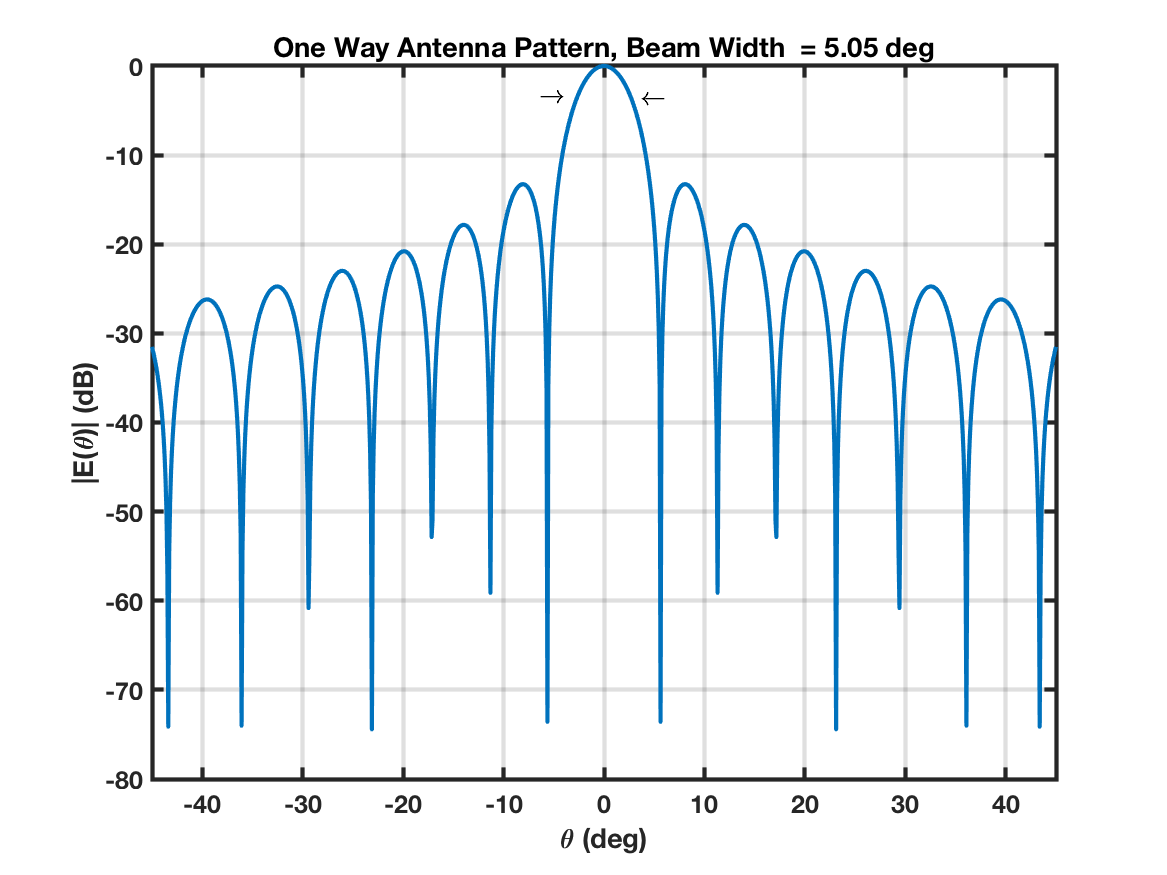
\includegraphics[width=4in]{../media/multistatic/sinc_antenna_pattern_one_way.png}
  \end{center}
  \renewcommand{\baselinestretch}{1} \small\normalsize
  \begin{quote}
    \caption[One Way Antenna Pattern]{One Way Antenna Pattern\label{rb_fig:4}}
  \end{quote}
\end{figure}
\renewcommand{\baselinestretch}{2} \small\normalsize

\subsection{Two Way}
The two way antenna beam width, $\theta_2$, is the beam width of the beam propagating in both directions. For the monostatic case, we can compute this as the one way beam width of the square of the antenna pattern. For the sinc pattern, the two way pattern is shown in Figure \ref{rb_fig:5}. In most cases, $\theta_2 \approx \frac{1}{\sqrt{2}}\theta$.

\begin{figure}[H]
  \begin{center}
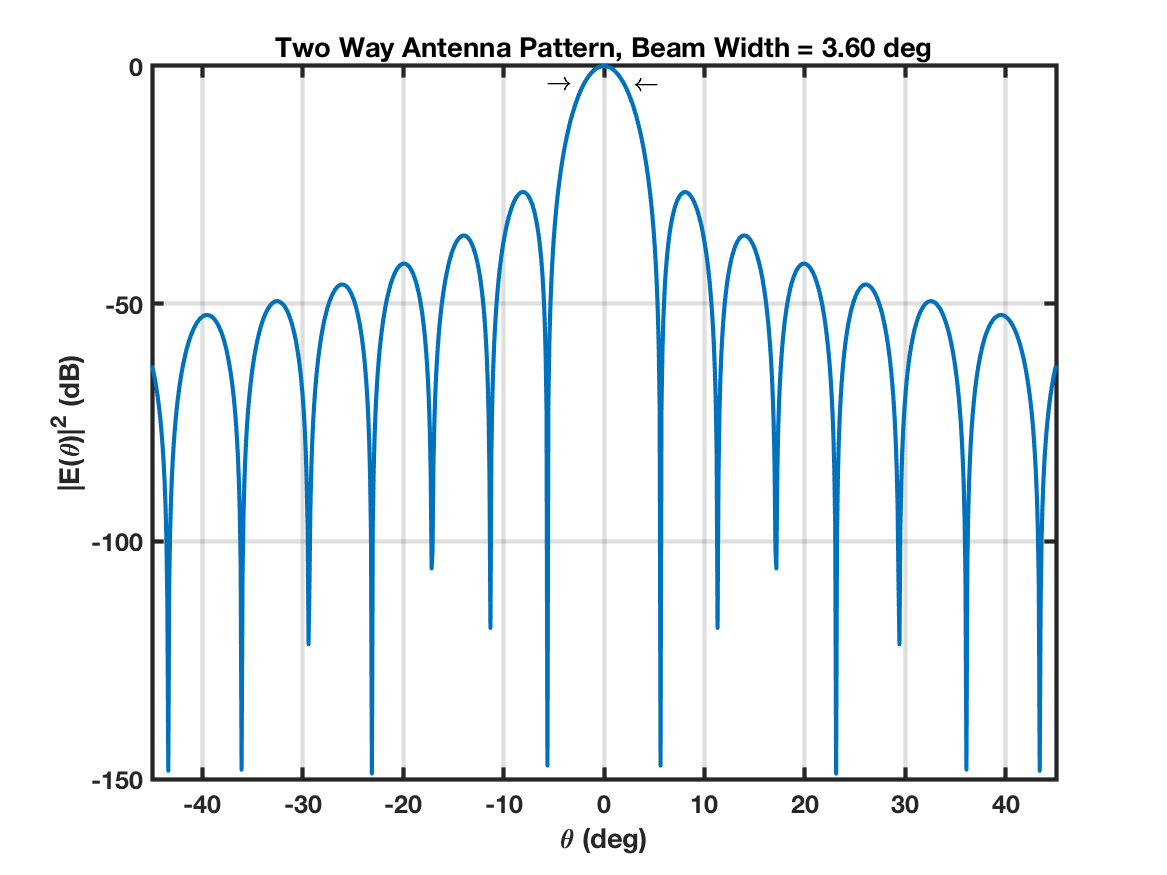
\includegraphics[width=4in]{../media/multistatic/sinc_antenna_pattern_two_way.png}
  \end{center}
  \renewcommand{\baselinestretch}{1} \small\normalsize
  \begin{quote}
    \caption[Two Way Antenna Pattern]{Two Way Antenna Pattern\label{rb_fig:5}}
  \end{quote}
\end{figure}
\renewcommand{\baselinestretch}{2} \small\normalsize
The two way beam width is really only valid for monostatic configurations that assume the forward and backward propagating beams lie directly on top of one another. In a bistatic configuration, the beams overlap differently and need to be explicitly evaluated.


\section{Detection}
The detection process can be cast as a hypothesis test where the two mutually exclusive hypotheses are that the target is either present or not present \cite{richards_radar}. There are three probabilities that need to be considered. First, the probability of detection, $P_d$, is the probability that a target is both detected and present. Second, the probability of false alarm, $P_{fa}$ is the probability that a target is detected but not actually present. Finally, the probability of miss, $P_m$ is the probability that a target is present but not detected. In most cases, a missed detection is worse than a false alarm.

\subsection{Threshold Testing}
The detection processes is generally a threshold test applied to the output of a matched filter with the threshold, $\hat{T}$ tuned to achieve a specified $P_{fa}$. Matched filters match the filter impulse response to the waveform to maximize the SNR and optimize detection \cite{richards_dsp}. 

The received signal consists of thermal noise, potential target returns, and potential interference signals such as clutter or jamming. Expressions for $P_d$ are complicated but well studied for the standard cases of Gaussian noise and fluctuating targets following Swerling models. As a general rule of thumb, an SNR of $13$ dB provides a $P_d$ of $\approx 0.94$ and a $P_{fa}$ of $\approx 10^{-6}$.

\subsection{Processing Gains}
To improve the overall SNR and increase the $P_d$, we can take advantage of processing gains by applying the detection strategy to groups of pulses. This is known as pulse integration and we can apply it coherently or noncoherently. We can also look at binary integration strategies where a detection is asserted for $M$ observations out of $N$ chances.

\subsubsection{Coherent and Noncoherent Integration}
For coherent integration, we operate in the complex domain and add the magnitude and phase of each pulse. The number of pulses, $N$, that are combined is defined as the Coherent Processing Interval (CPI) and the overall processing gain goes as $N^2$.

For noncoherent integration, we only sum the magnitudes of each pulse. We now refer to the number of pulses combined, $N$, as the Noncoherent Processing Interval (NPI) and the overall processing gain goes as $N$. When using noncoherent integration, sometimes the NPI is still referred to as the CPI.

Coherently integration $2$ pulses provides a $6$ dB processing gain while noncoherently integrating $2$ pulses only provides a $3$ dB processing gain.

\subsubsection{Binary Integration}
Binary integration relies on cumulative probability to improve $P_d$ and reduce $P_{fa}$. For the specific strategy of requiring $M$ positive hits out of $N$ observations to claim a detection, the improvement in probability is given in Equation \ref{rb_eq:2} where $P$ is the resulting probability and $p$ is the single opportunity probability (either $P_d$ or $P_{fa}$). 

\begin{equation}
\label{rb_eq:2}
P = \sum_{r=M}^N\binom{N}{k}p^k\left(1-p \right)^{N-k}
\end{equation}

The standard $N$ choose $k$ from Equation \ref{rb_eq:2} is given by:
\begin{equation}
\label{rb_eq:3}
\binom{N}{k} = \frac{N!}{(N-k)!k!}
\end{equation}